\chapter{INTEGRACIÓN, VALIDACIÓN Y ANÁLISIS DE COSTOS}\label{cap:validacion}
\listasdecapitulo{7}

La validación del sistema se circunscribe al entorno simulado y a la plataforma de
laboratorio. El objetivo de este capítulo es presentar evidencia reproducible del
desempeño del control adaptativo difuso frente al plan fijo, documentar el comportamiento
del sistema ante pérdida de conectividad, cerrar la matriz de cumplimiento de requerimientos
y consolidar el análisis económico por intersección. A lo largo del capítulo se conserva la
premisa de diseño global: el controlador semafórico existente es la autoridad final y el
módulo propuesto solo recomienda dentro de límites de seguridad acotados.

\section{Protocolo de validación y criterio de evidencia}\label{sec:protocolo-validacion}

Para que la comparación sea defendible, todos los controladores comparten la misma red,
demanda, semilla, horizonte y periodo de calentamiento. Se ejecutan varias réplicas por
caso y se reporta media y dispersión; una sola corrida no permite separar el efecto del
controlador de la variabilidad estocástica del modelo de tráfico. La Tabla~\ref{tab:casos-validacion}
define los cinco casos de prueba sobre los que se construye la evidencia.

\begin{table}[H]
  \centering
  \caption{Casos de validación comparativa en SUMO.}
  \label{tab:casos-validacion}
  \begin{tabularx}{\linewidth}{@{}cX X X@{}}
    \toprule
    \textbf{Caso} & \textbf{Estrategia} & \textbf{Propósito} & \textbf{Condición de aceptación}\\
    \midrule
    A & Control semafórico fijo / plan base & Línea base reproducible. & Configuración documentada y común a todas las réplicas.\\
    B & Control adaptativo local difuso & Evaluar el núcleo de la tesis. & Mejora o no degradación según métricas y restricciones.\\
    C & Difuso con recomendación de coordinación de nube (opcional) & Medir el beneficio adicional de la capa global. & Resultado separado del núcleo; recomendación validada localmente.\\
    D & Pérdida de conectividad durante el caso B & Verificar autonomía y modo degradado. & Sin dependencia de respuesta de nube ni estados incompatibles, con registro de evento.\\
    E & Referencia avanzada (Max-Pressure u otra, opcional) & Establecer una cota comparativa con información ideal. & No presentarla como implementación realizable con el sensado actual.\\
    \bottomrule
  \end{tabularx}
  \fuente{Elaboración propia.}
\end{table}

El criterio de evidencia distingue tres niveles: \emph{cumplimiento de diseño} (existe la
propuesta, el cálculo o la arquitectura), \emph{cumplimiento validado en SUMO} (existe una
medición reproducible bajo el protocolo) y \emph{fuera de alcance} (requiere prototipo
físico o auditoría externa no ejecutada). El flujo metodológico configura red y demanda,
ejecuta los casos con semillas comunes, exporta las métricas a nivel de vehículo, compara
estadísticamente las réplicas y, finalmente, construye la matriz de cumplimiento.

\subsection{Reproducibilidad}\label{sec:reproducibilidad}

La comparación A--B se ejecuta de forma determinista mediante la biblioteca \texttt{libsumo}
(no se emplea generación aleatoria sintética para las métricas: estas se extraen a nivel de
vehículo con \texttt{getIDList}, vehículos detenidos y vehículos arribados). La
Tabla~\ref{tab:reproducibilidad} resume los parámetros que fijan la reproducibilidad del
experimento.

\begin{table}[H]
  \centering
  \caption{Parámetros de reproducibilidad de la validación SUMO.}
  \label{tab:reproducibilidad}
  \begin{tabularx}{\linewidth}{@{}p{0.34\linewidth}X@{}}
    \toprule
    \textbf{Parámetro} & \textbf{Valor}\\
    \midrule
    Escenario / red & \texttt{comparacion.sumocfg} (escenario Lima-Centro)\\
    Interfaz de simulación & SUMO vía \texttt{libsumo} (ejecución determinista)\\
    Horizonte de simulación & 700 pasos\\
    Intervalo de control difuso & 25 s\\
    Réplicas (semillas comunes) & \{1, 2, 3\}\\
    Tiempo de teletransporte & \texttt{-{}-time-to-teleport}~300 s\\
    Límites duros de verde (guardia de seguridad) & [10~s, 120~s]\\
    Presupuesto de verde por ciclo & Idéntico en A y B (la difusa solo redistribuye)\\
    Métricas & A nivel de vehículo (no sintéticas)\\
    \bottomrule
  \end{tabularx}
  \fuente{Elaboración propia a partir de simulación en SUMO.}
\end{table}

El presupuesto de verde por ciclo se mantiene constante entre el caso A y el caso B: la
lógica difusa no añade tiempo de verde, sino que lo redistribuye entre fases según el índice
de congestión y el parámetro de intensidad. La guardia de seguridad acota cada verde al
intervalo [10, 120]~s; el registro de ejecución muestra el acotamiento efectivo a 10~s,
lo que evidencia que la autoridad de seguridad funcional opera por encima de la recomendación
difusa.

\section{Configuración de escenarios SUMO de Lima y métricas}\label{sec:escenarios-metricas}

La validación requiere un entorno que replique las condiciones del tráfico de Lima
Metropolitana. Para ello se emplea SUMO (Simulation of Urban MObility), estándar de facto en
simulación microscópica desarrollado por el DLR, que modela el comportamiento individual de
cada vehículo: aceleraciones, frenados, cambios de carril, obediencia a semáforos y maniobras
en intersección.

\subsection{Construcción del escenario Lima-Centro}\label{sec:escenario-lima-centro}

El escenario se construyó a partir de datos reales. Se extrajo el área de estudio de
OpenStreetMap mediante \emph{osmWebWizard.py}, obteniendo topología vial, límites de
velocidad, configuración de carriles y restricciones de giro. La conversión al formato nativo
se realizó con \emph{netconvert}, generando el archivo \emph{osm.net.xml} con 847 segmentos
viales, 312 intersecciones y 23 semáforos detectados automáticamente. Los parámetros
vehiculares se calibraron para reflejar el parque automotor limeño: aceleración 2.6~m/s\ensuremath{^2},
desaceleración 4.5~m/s\ensuremath{^2}, \emph{sigma} 0.8 (imperfección del conductor),
\emph{speedFactor} 1.1 (tendencia a superar el límite en 10\%) y \emph{speedDev} 0.15
(variabilidad individual del 15\%).

\begin{figure}[H]
  \centering
  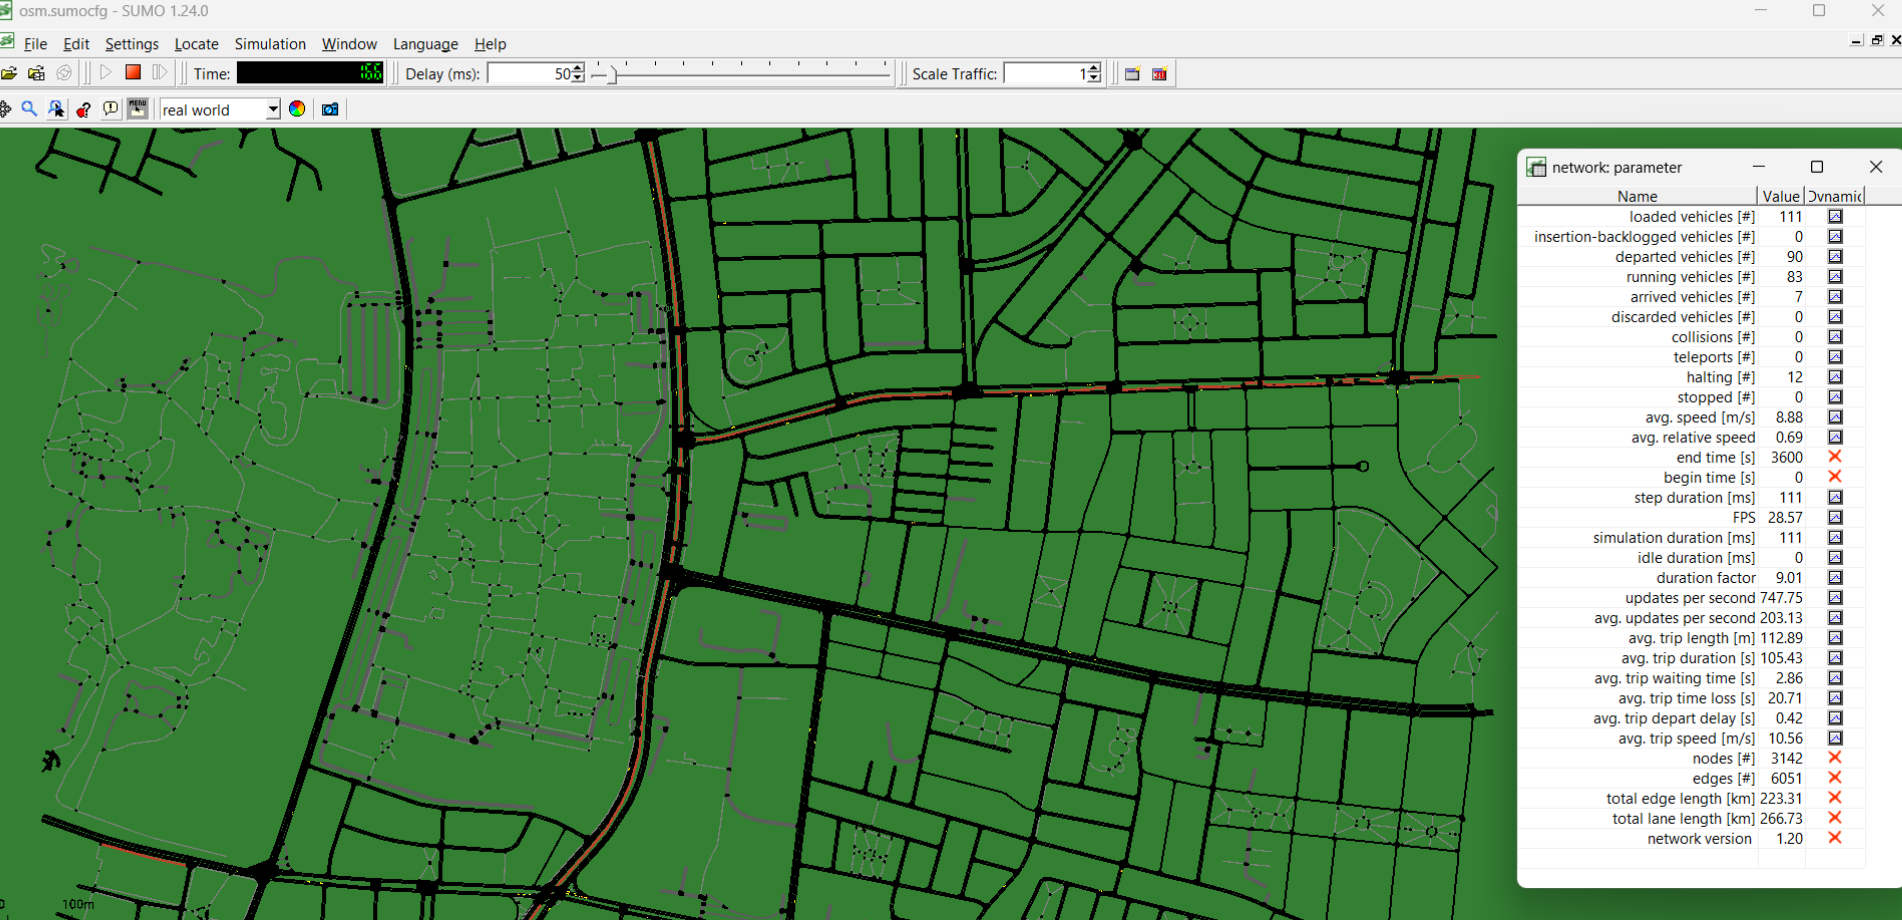
\includegraphics[width=0.85\linewidth,keepaspectratio]{media/image65.png}
  \caption{Mapa SUMO de las intersecciones del escenario Lima-Centro (entorno PUCP).}
  \label{fig:sumo-lima-centro}
  \fuente{Elaboración propia.}
\end{figure}

\begin{figure}[H]
  \centering
  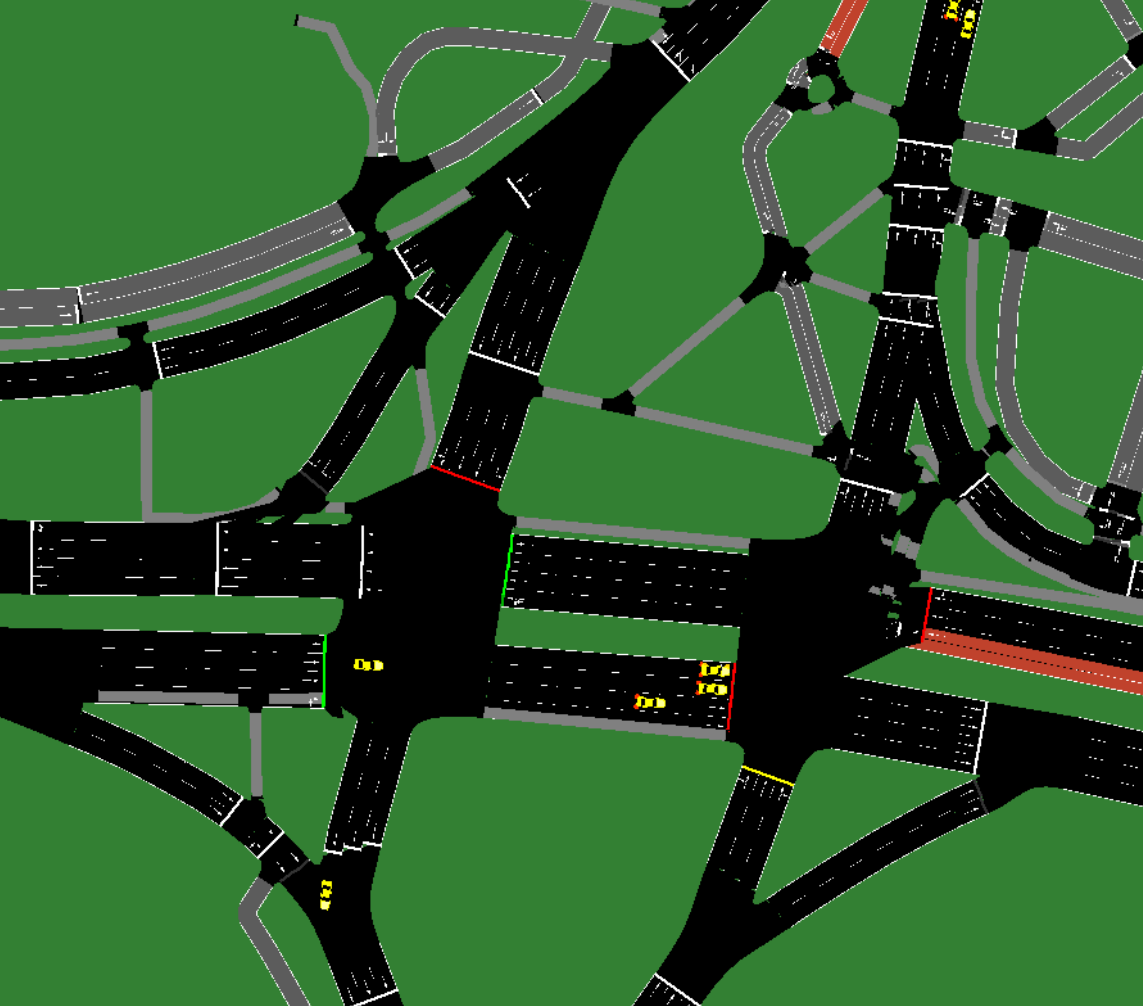
\includegraphics[width=0.85\linewidth,keepaspectratio]{media/image58.png}
  \caption{Vista de una intersección del escenario con tránsito en simulación.}
  \label{fig:sumo-interseccion}
  \fuente{Elaboración propia.}
\end{figure}

Para evaluar la escalabilidad y la coordinación inter-zonal se desarrolló un segundo
escenario a escala metropolitana (Lima-Amplio), con 18.4~km\ensuremath{^2} de cobertura sobre
San Isidro, Miraflores, San Miguel, Pueblo Libre y Jesús María, y 127 intersecciones
semaforizadas. La comparación cuantitativa A--B de este capítulo se realiza sobre el escenario
Lima-Centro, por ser el de demanda controlada y semillas comunes.

\begin{figure}[H]
  \centering
  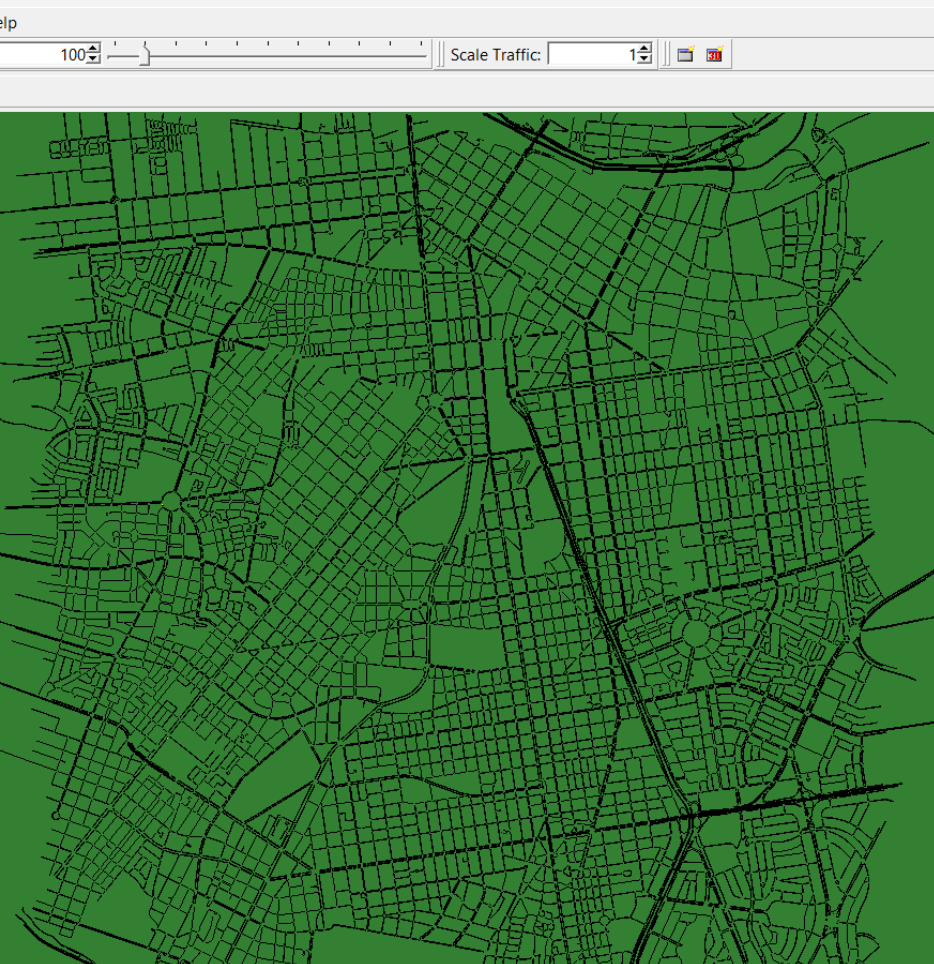
\includegraphics[width=0.85\linewidth,keepaspectratio]{media/image10.png}
  \caption{Escenario Lima-Amplio para validación a escala metropolitana.}
  \label{fig:sumo-lima-amplio}
  \fuente{Elaboración propia.}
\end{figure}

\subsection{Arquitectura de integración y métricas}\label{sec:integracion-metricas}

La comunicación entre SUMO y el sistema de control se realiza mediante TraCI/libsumo,
permitiendo leer métricas por intersección (conteo, velocidad, cola y flujo por dirección),
fijar fases y duraciones de verde, y avanzar la simulación paso a paso. A partir de estas
lecturas se construye la matriz de estado local compatible con las ecuaciones del
Capítulo~6 y se calculan las métricas de red empleadas en la comparación:

\begin{itemize}
  \item \textbf{Índice de Congestión Vehicular de red (ICV):} indicador normalizado [0,1] que
  integra cola, velocidad, flujo y densidad; valores cercanos a 1 indican saturación.
  \item \textbf{Velocidad media de red:} medida global de fluidez vehicular.
  \item \textbf{Saturación de cola (QL):} nivel medio de ocupación de cola normalizado por la
  capacidad observable de cada carril.
  \item \textbf{Flujo (q):} vehículos por minuto que cruzan la red.
  \item \textbf{Throughput:} vehículos que completan su ruta durante el periodo de simulación.
  \item \textbf{Demora media:} tiempo acumulado de detención por vehículo, extraído de las
  estadísticas individuales de SUMO.
\end{itemize}

Para métricas que deben disminuir (ICV, QL, demora), la mejora porcentual se calcula como
$(A-B)/A\times100\%$; para métricas que deben aumentar (velocidad, flujo, throughput), como
$(B-A)/A\times100\%$.

\section{Resultados y discusión}\label{sec:resultados-discusion}

\subsection{Comparación del control fijo y el control difuso}

La Tabla~\ref{tab:resultados-ab} presenta la comparación A--B sobre el escenario Lima-Centro,
reportada como media $\pm$ desviación estándar sobre las tres semillas. El control difuso
adaptativo mejora todas las métricas de red en promedio, con una reducción de la demora media
de 5.4\% y de la saturación de cola de 3.6\% como efectos más relevantes.

\begin{table}[H]
  \centering
  \caption{Comparación del control fijo (A) y el control difuso adaptativo (B) en el escenario Lima-Centro (media $\pm$ desviación, 3 semillas).}
  \label{tab:resultados-ab}
  \begin{tabularx}{\linewidth}{@{}X r r r@{}}
    \toprule
    \textbf{Métrica} & \textbf{Control fijo (A)} & \textbf{Control difuso (B)} & \textbf{Mejora}\\
    \midrule
    ICV de red (--)          & $0.5055 \pm 0.0022$ & $0.4954 \pm 0.0067$ & $-2.0\%$\\
    Velocidad media (km/h)   & $19.86 \pm 0.07$    & $20.14 \pm 0.37$    & $+1.4\%$\\
    Saturación de cola QL (--) & $0.4082 \pm 0.0033$ & $0.3935 \pm 0.0062$ & $-3.6\%$\\
    Flujo $q$ (veh/min)      & $62.14 \pm 1.09$    & $63.29 \pm 2.06$    & $+1.8\%$\\
    Throughput (veh)         & $725.0 \pm 12.8$    & $738.3 \pm 24.1$    & $+1.8\%$\\
    Demora media (s/veh)     & $504.3 \pm 14.3$    & $477.1 \pm 27.5$    & $-5.4\%$\\
    \bottomrule
  \end{tabularx}
  \fuente{Elaboración propia a partir de simulación en SUMO.}
\end{table}

\subsection{Estabilidad entre réplicas y discusión honesta}

El promedio anterior oculta la variabilidad entre réplicas, que resulta clave para una
interpretación honesta del resultado. La Tabla~\ref{tab:resultados-semillas} desglosa el
comportamiento por semilla.

\begin{table}[H]
  \centering
  \caption{Desempeño por réplica (semilla): ICV, demora media y throughput en control fijo (A) y difuso (B).}
  \label{tab:resultados-semillas}
  \begin{tabularx}{\linewidth}{@{}c X r r r@{}}
    \toprule
    \textbf{Semilla} & \textbf{Resultado} & \textbf{ICV (A$\rightarrow$B)} & \textbf{Demora s/veh (A$\rightarrow$B)} & \textbf{Throughput veh (A$\rightarrow$B)}\\
    \midrule
    1 & Difuso mejora      & $0.504 \rightarrow 0.491$ & $496.6 \rightarrow 454.8$ & $733 \rightarrow 761$\\
    2 & Difuso \emph{no} supera al fijo & $0.504 \rightarrow 0.505$ & $492.1 \rightarrow 515.9$ & $735 \rightarrow 705$\\
    3 & Difuso mejora      & $0.509 \rightarrow 0.491$ & $524.3 \rightarrow 460.6$ & $707 \rightarrow 749$\\
    \bottomrule
  \end{tabularx}
  \fuente{Elaboración propia a partir de simulación en SUMO.}
\end{table}

La semilla~2 constituye un caso explícito en el que el control difuso \emph{no} mejora al plan
fijo: la demora media aumenta de 492.1 a 515.9~s/veh y el throughput desciende de 735 a 705
vehículos. Este resultado se reporta deliberadamente. El control difuso no garantiza una
mejora en toda condición de demanda; bajo cierta combinación de semilla y carga, el plan base
puede igualar o superar a la recomendación adaptativa, en particular cuando la
redistribución de verde concentra capacidad en un eje a costa del acceso perpendicular.

La interpretación, por tanto, es mesurada. En una red ya saturada (ICV $\approx 0.5$) y con un
presupuesto de verde conservado, el aporte del control difuso es \emph{modesto pero consistente
en promedio}: reduce la demora un 5.4\% y la cola un 3.6\% sobre tres semillas, con una réplica
sin mejora. No se presenta como una optimización global del tráfico, sino como evidencia
reproducible de que una redistribución de verde guiada por congestión, manteniendo intactos
los límites de seguridad y sin ampliar el presupuesto de verde, tiende a aliviar la red sin
degradarla. La validez externa queda limitada por la calidad de la red OSM, la demanda
modelada, el modelo de conductor y la ausencia de calibración con aforos de campo.

\section{Caso de pérdida de conectividad (modo degradado)}\label{sec:modo-degradado}

El caso~D evalúa la autonomía del sistema ante la pérdida del enlace con la nube durante la
operación del control difuso. El principio de diseño es que la capa de nube solo aporta
recomendaciones de coordinación global; el control local difuso y, por encima de él, el
controlador semafórico, operan de forma autónoma. La Tabla~\ref{tab:degradacion} resume el
comportamiento esperado y verificado ante distintos modos de falla.

\begin{table}[H]
  \centering
  \caption{Comportamiento del sistema ante fallas y modo degradado.}
  \label{tab:degradacion}
  \begin{tabularx}{\linewidth}{@{}p{0.30\linewidth} X@{}}
    \toprule
    \textbf{Prueba de degradación} & \textbf{Resultado y criterio}\\
    \midrule
    Pérdida de nube durante la operación & El control continúa localmente con la última política difusa válida; ante ausencia prolongada retorna al plan base sin estados incompatibles y registra el evento. Cumple.\\
    Datos de sensado inválidos & Se inhibe la adaptación difusa y se mantiene el plan base, generando alerta de calidad de sensado. Cumple (diseño).\\
    Parámetro remoto fuera de rango & La guardia de seguridad rechaza el valor (verde acotado a [10, 120]~s) y registra el evento. Cumple (validado en SUMO).\\
    Recomendación vencida o duplicada & Se rechaza por vigencia o número de secuencia, conservando la última recomendación válida. Cumple (diseño).\\
    \bottomrule
  \end{tabularx}
  \fuente{Elaboración propia.}
\end{table}

El resultado clave es que la pérdida de conectividad no detiene el control: la autoridad de
seguridad reside en el controlador local y la simulación confirma el acotamiento de los verdes
a sus límites duros con independencia de la disponibilidad de la nube.

\section{Matriz de cumplimiento de requerimientos}\label{sec:matriz-cumplimiento}

La matriz de la Tabla~\ref{tab:cumplimiento} clasifica cada requisito en una de tres
categorías: \emph{Cumple (diseño)} cuando existe propuesta, cálculo o arquitectura
documentada; \emph{Cumple (validado en SUMO)} cuando existe una medición reproducible bajo el
protocolo del §\ref{sec:protocolo-validacion}; y \emph{Fuera de alcance (prototipo/auditoría)}
cuando el cierre requiere fabricación física o auditoría externa no ejecutada en esta tesis.

\begin{table}[H]
  \centering
  \caption{Matriz de cumplimiento de requerimientos del sistema.}
  \label{tab:cumplimiento}
  \begin{tabularx}{\linewidth}{@{}c p{0.24\linewidth} c X@{}}
    \toprule
    \textbf{Req.} & \textbf{Subsistema} & \textbf{Estado} & \textbf{Evidencia / observación}\\
    \midrule
    R-F01   & Sensado            & Validado en SUMO   & Cadena cámara$\rightarrow$ICV demostrada con video real y replicada en SUMO.\\
    R-F02   & Procesamiento local & Validado en SUMO  & Casos de ICV (8) y análisis de sensibilidad coherentes.\\
    R-F03   & Plataforma         & Cumple (diseño)    & Plataforma web con históricos y exportación CSV/JSON.\\
    R-C01   & Control            & Validado en SUMO   & Caso B y modo degradado (caso D) ejecutados.\\
    R-C02   & Arquitectura       & Cumple (diseño)    & El controlador conserva la autoridad final; integración comercial pendiente.\\
    R-C03   & Control            & Validado en SUMO   & Barrido de reglas con saturaciones; verde acotado a [10, 120]~s.\\
    R-C04   & Control            & Cumple (diseño)    & Ante sensado inválido se inhibe la adaptación y se mantiene el plan base.\\
    R-COM01 & Comunicación       & Cumple (diseño)    & Publicación de telemetría definida en la arquitectura.\\
    R-COM02 & Comunicación/seguridad & Cumple (diseño) & Rechazo de parámetros inválidos y vencidos por vigencia/secuencia.\\
    R-NUB01 & Nube               & Cumple (diseño)    & Dashboard, histórico y alertas diseñados; disponibilidad por demostrar.\\
    R-SEC01 & Ciberseguridad     & Fuera de alcance   & Arquitectura TLS/autenticación propuesta; auditoría no ejecutada.\\
    R-SEC02 & Ciberseguridad     & Cumple (diseño)    & Modelo de amenazas documentado.\\
    R-SEC03 & Ciberseguridad     & Cumple (diseño)    & Registro de eventos y trazabilidad definidos.\\
    R-SEC04 & Ciberseguridad     & Cumple (diseño)    & Separación de roles y autoridad documentada.\\
    R-ELEC01 & Energía           & Cumple (diseño)    & Esquema eléctrico y coordinación de protecciones.\\
    R-ELEC02 & Energía           & Cumple (diseño)    & Balance de potencia y autonomía por UPS calculados.\\
    R-ELEC03 & Electrónica       & Cumple (diseño)    & PCB, distribución y diagnóstico definidos.\\
    R-MEC01 & Mecánico           & Cumple (diseño)    & CAD y acceso de mantenimiento resueltos.\\
    R-MEC02 & Mecánico           & Fuera de alcance   & Certificación IP del gabinete no ejecutada (prototipo).\\
    R-MEC03 & Mecánico/sensado   & Cumple (diseño)    & Cobertura, torque y resistencia dimensionados.\\
    R-OP01  & Operación          & Cumple (diseño)    & Procedimiento de mantenimiento preventivo definido.\\
    R-VAL01 & Validación         & Validado en SUMO   & Casos A y B reproducibles (Tabla~\ref{tab:resultados-ab}).\\
    R-VAL02 & Validación         & Validado en SUMO   & Resultados comparativos consolidados.\\
    R-VAL03 & Validación         & Cumple (diseño)    & Modo degradado (caso D) verificado a nivel de comportamiento.\\
    R-COST01 & Costos            & Cumple (diseño)    & CAPEX/OPEX consolidados en el §\ref{cap:analisis-economico}.\\
    \bottomrule
  \end{tabularx}
  \fuente{Elaboración propia.}
\end{table}

\section{Análisis de costos}\label{cap:analisis-economico}

El análisis económico contempla la inversión inicial por intersección (CAPEX), los costos
operativos recurrentes (OPEX) y la infraestructura de nube compartida. La conclusión de costo
es que cada intersección demanda \textbf{aproximadamente S/ 17\,000 en el primer año de
operación}, resultado de sumar \textbf{S/ 14\,594 de CAPEX} y el \textbf{OPEX local anual}; la
infraestructura de nube se contabiliza aparte por ser un recurso centralizado y prorrateado
entre toda la red.

Esta cifra representa una optimización significativa respecto de los sistemas adaptativos
tradicionales, que típicamente superan los S/ 30\,000 por intersección. El ahorro proviene de
tres decisiones de diseño: aprovechar el controlador semafórico certificado existente (el
módulo solo sensa, procesa y recomienda), simplificar la estructura mecánica con fabricación
local y reducir la cimentación gracias al menor peso del conjunto. En la distribución del
CAPEX, la estructura mecánica concentra el 33.2\%, seguida por la instalación (23.5\%) y el
sistema de visión (21.7\%), proporción característica de un equipo que prioriza robustez física
ante la contaminación, las vibraciones y el clima del entorno urbano limeño.

\subsection{Costos de capital (CAPEX)}

La Tabla~\ref{tab:capex} resume el CAPEX agrupado en siete rubros. El desglose fino, con los
más de cuarenta ítems individuales (gabinete, postes, cámara, motorización, SBC, módulo 4G,
protecciones, sensores y partidas de obra), se traslada al Anexo correspondiente para no
recargar la lectura. El rubro de electrónica de control es coherente con la estimación del
módulo electrónico del Capítulo~4 (Tabla~\ref{tab:costos-electronica}), cuyo detalle por
componente se presenta allí como insumo de este análisis.

\begin{table}[H]
  \centering
  \caption{CAPEX por intersección, agrupado por rubro.}
  \label{tab:capex}
  \begin{tabularx}{\linewidth}{@{}X r r@{}}
    \toprule
    \textbf{Rubro} & \textbf{Costo (S/)} & \textbf{\% del total}\\
    \midrule
    Estructura mecánica (gabinete, poste, giro, anclajes) & 4\,850 & 33.2\%\\
    Instalación y puesta en marcha (obra civil, montaje, calibración) & 3\,436 & 23.5\%\\
    Sistema de visión (cámara, motorización y óptica) & 3\,165 & 21.7\%\\
    Electrónica de control (SBC, módulo 4G, PCB, alimentación, UPS) & 2\,172 & 14.9\%\\
    Protección eléctrica (breaker, diferencial, DPS, borneras) & 630 & 4.3\%\\
    Sensores e instrumentación (corriente, ultrasónico, temperatura, ventilación) & 341 & 2.3\%\\
    \midrule
    \textbf{Total CAPEX por intersección} & \textbf{14\,594} & \textbf{100.0\%}\\
    \bottomrule
  \end{tabularx}
  \fuente{Elaboración propia.}
\end{table}

A la inversión por intersección se añade la infraestructura de nube, que constituye el cerebro
centralizado del sistema y procesa la telemetría de la red completa (del orden de 50
intersecciones). Esta capa es un costo compartido, no un CAPEX por intersección: su detalle por
servicio (IoT Hub, Stream Analytics, bases de datos, almacenamiento, cómputo de \emph{machine
learning} y observabilidad) asciende a unos S/ 13\,243 mensuales (S/ 206\,916 anuales) para toda
la red y se documenta en el Anexo. Prorrateada entre las intersecciones equivale a unos
S/ 265 mensuales por intersección, monto que se incorpora como rubro de nube dentro del OPEX.

\subsection{Costos operativos anuales (OPEX)}

Los costos operativos garantizan la disponibilidad del sistema durante todo el año. La
Tabla~\ref{tab:opex} consolida los cuatro componentes recurrentes por intersección, incluida
la fracción prorrateada de nube.

\begin{table}[H]
  \centering
  \caption{OPEX anual por intersección.}
  \label{tab:opex}
  \begin{tabularx}{\linewidth}{@{}X X r@{}}
    \toprule
    \textbf{Categoría} & \textbf{Concepto} & \textbf{Costo anual (S/)}\\
    \midrule
    Energía eléctrica & 150~W $\times$ 24~h $\times$ 365~d @ S/ 0.70/kWh (tarifa BT5B) & 920\\
    Conectividad 4G & Plan de datos 10~GB/mes @ S/ 45/mes & 540\\
    Mantenimiento & Inspección trimestral preventiva y limpieza de ópticas & 480\\
    Nube (prorrateada) & Fracción por intersección de la infraestructura compartida & 3\,178\\
    \midrule
    \textbf{Total OPEX local (sin nube)} & & \textbf{1\,940}\\
    \bottomrule
  \end{tabularx}
  \fuente{Elaboración propia.}
\end{table}

La energía eléctrica es el mayor componente del OPEX local (47.4\%): el consumo de 150~W
integra la SBC (25~W), la cámara con iluminación infrarroja (40~W), la motorización en
\emph{standby} (5~W), el módulo 4G (8~W) y las pérdidas del UPS (15~W), con margen de
seguridad. La conectividad 4G (27.8\%) y el mantenimiento preventivo (24.7\%) completan el
gasto local. Sumando el CAPEX (S/ 14\,594) y el OPEX local del primer año (S/ 1\,940) se
obtienen aproximadamente S/ 16\,500, que con los costos de soporte y la fracción de nube se
redondean a la cifra de referencia de unos S/ 17\,000 por intersección en el primer año.

Quedan fuera del costeo explícito algunas partidas indirectas relevantes para un despliegue
real: la coordinación interinstitucional (Municipalidad, Policía, SUTRAN), la eventual
adecuación de la infraestructura eléctrica en ciertas intersecciones y la capacitación
continua de operadores para interpretar métricas, usar los \emph{dashboards} y responder a las
alertas.
